\begingroup
	\pgfdeclarelayer{background layer}
	\pgfsetlayers{background layer,main}
	\tikzstyle{zero}=[circle,draw=black,fill=white,inner sep=0pt,minimum size=2.5mm]
	\tikzstyle{one}=[circle,draw=black,fill=black,inner sep=0pt,minimum size=2.5mm]
	\tikzstyle{two}=[circle,draw=black,fill=gray,inner sep=0pt,minimum size=2.5mm]
		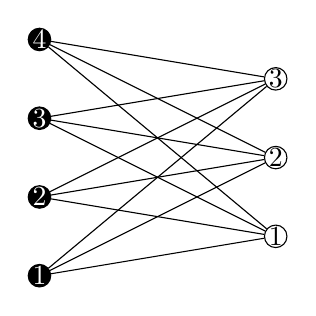
\begin{tikzpicture}
			\foreach \t in {1,2,3,4}
			{
				\node [white] (\t) at  (1,\t) [one] {$\t$};
			}
			\foreach \t/\l in {1/A,2/B,3/C}
			{
				\node (\l) at  (4,\t+.5) [zero] {$\t$};
			}
			\foreach \x in {1,2,3,4}
			\foreach \l in {A,B,C}
			\draw (\x)--(\l);	
		\end{tikzpicture}
	%\label{fig:eg_k_3_4}	
\endgroup